%%%%%%%%%%%%%%%%%%%%%%%%%%%%%%%%%%%%%%%%%
% Student: Francis Pruter
% Assignment 1
% CS 595
%
% used the template from:
% http://www.latextemplates.com/template/structured-general-purpose-assignment
%%%%%%%%%%%%%%%%%%%%%%%%%%%%%%%%%%%%%%%%%

%----------------------------------------------------------------------------------------
%	PACKAGES AND OTHER DOCUMENT CONFIGURATIONS
%----------------------------------------------------------------------------------------

\documentclass{article}
\setlength{\paperheight}{11in}

\usepackage{fancyhdr} % Required for custom headers
\usepackage{lastpage} % Required to determine the last page for the footer
\usepackage{extramarks} % Required for headers and footers
\usepackage{graphicx} % Required to insert images
\usepackage{listings} % Required to insert codes

% Margins
\topmargin=-0.45in
\evensidemargin=0in
\oddsidemargin=0in
\textwidth=6.5in
\textheight=9.0in
\headsep=0.25in 

\linespread{1.1} % Line spacing

% Set up the header and footer
\pagestyle{fancy}
\lhead{\hmwkAuthorName} % Top left header
\chead{\hmwkClass\ (\hmwkClassInstructor\ \hmwkClassTime): \hmwkTitle} % Top center header
\rhead{\firstxmark} % Top right header
\lfoot{\lastxmark} % Bottom left footer
\cfoot{} % Bottom center footer
\rfoot{Page\ \thepage\ of\ \pageref{LastPage}} % Bottom right footer
\renewcommand\headrulewidth{0.4pt} % Size of the header rule
\renewcommand\footrulewidth{0.4pt} % Size of the footer rule

\setlength\parindent{0pt} % Removes all indentation from paragraphs

   
%----------------------------------------------------------------------------------------
%	NAME AND CLASS SECTION
%----------------------------------------------------------------------------------------

\newcommand{\hmwkTitle}{Assignment\ \#1} % Assignment title
\newcommand{\hmwkDueDate}{Thursday,\ September\ 11,\ 2014} % Due date
\newcommand{\hmwkClass}{CS\ 595} % Course/class
\newcommand{\hmwkClassTime}{04:20pm} % Class/lecture time
\newcommand{\hmwkClassInstructor}{MLN} % Teacher/lecturer
\newcommand{\hmwkAuthorName}{Francis W. Pruter, Jr.} % Your name

\begin{document}         
% Start your text
\section{Problem 1:}
\label{Problem 1}

{\bf Demonstrate that you know how to use "curl" well enough to
correctly POST data to a form.  Show that the HTML response that
is returned is "correct".  That is, the server should take the
arguments you POSTed and build a response accordingly.  Save the
HTML response to a file and then view that file in a browser and
take a screen shot.
\newline
} 

{\it Below is the Bash code used to POST data to www.stubhub.com to find an event matching "Hokies".  -A is used to declare the UserAgent as Firefox.  -F is for field to be posted. -v is for more output. -o is used to make the output file to save the response.html}
\begin{lstlisting}[language=Bash,frame=single,caption=Curl, 
                 label={CUrl}, breaklines=true]
curl -A "Firefox" -vF "searchStr=Hokies" "http://www.stubhub.com/search/doSearch" -o stubhub.html

\end{lstlisting}

{\it Below is the images of the output "stubhub.html"}

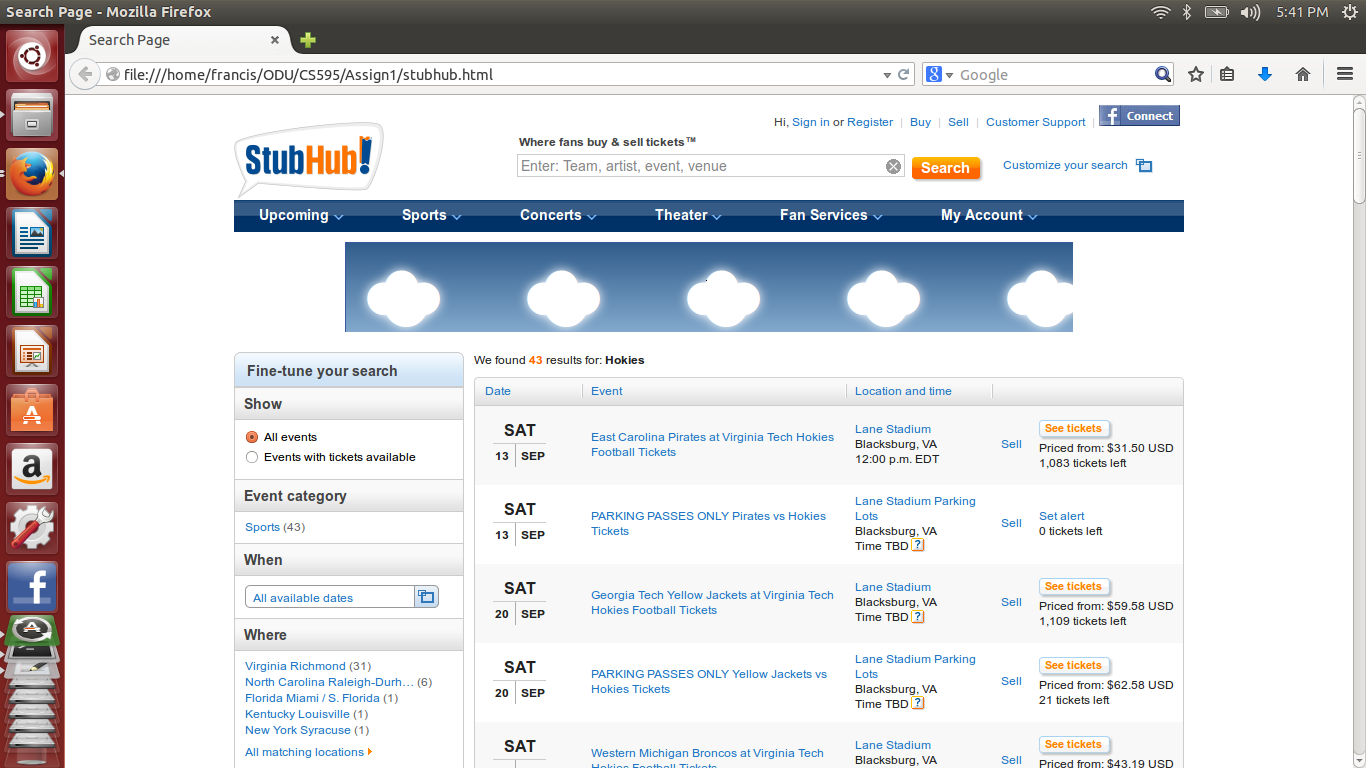
\includegraphics[width=\textwidth]{prob1}
\newpage
\section{Problem 2:}
\label{Problem 2}

{\bf Write a Python program that: \newline
  1. takes one argument, like "Old Dominion" or "Virginia Tech"\newline
  2. takes another argument specified in seconds (e.g., "60" for 
     one minute).
  3. takes a URI as a third argument: \newline
     http://sports.yahoo.com/college-football/scoreboard/ \newline
     or\newline
     http://sports.yahoo.com/college-football/scoreboard/?week=2\&conf=all\newline
     or\newline
     http://sports.yahoo.com/college-football/scoreboard/?week=1\&conf=72\newline
     etc.\newline
  4. dereferences the URI, finds the game corresponding to the team
     argument, prints out the current score (e.g., "Old Dominion 27, 
     East Carolina 17), sleeps for the specified seconds, and then
     repeats (until control-C is hit).\newline
} 

\lstinputlisting[language=Python,frame=single,caption=score.py, 
                 label={score.py}, breaklines=true]{score.py}



\begin{figure}[h!]
    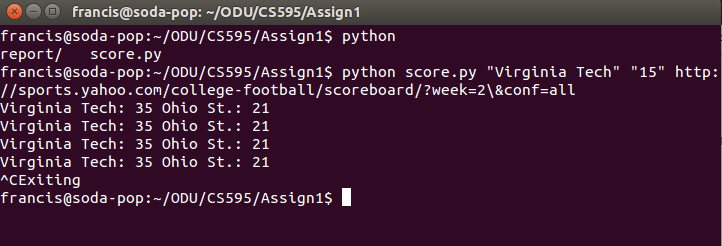
\includegraphics[width=\textwidth]{prob2_running}
    \caption{GO HOKIES!}
\end{figure}

\newpage
\section{Problem 3:}
\label{Problem 3}

{\bf Consider the "bow-tie" graph in the Broder et al. paper (fig 9):\newline
    http://www9.org/w9cdrom/160/160.html\newline
\newline
    Now consider the following graph:\newline
\newline

    A $\rightarrow$ B\newline
    B $\rightarrow$ C\newline
    C $\rightarrow$ D\newline
    C $\rightarrow$ A\newline
    C $\rightarrow$ G\newline
    E $\rightarrow$ F\newline
    G $\rightarrow$ C\newline
    G $\rightarrow$ H\newline
    I $\rightarrow$ H\newline
    I $\rightarrow$ J\newline
    I $\rightarrow$ K\newline
    J $\rightarrow$ D \newline
    L $\rightarrow$ D\newline
    M $\rightarrow$ A\newline
    M $\rightarrow$ N\newline
    N $\rightarrow$ D\newline
\newline    
    For the above graph, give the values for:
\newline
\newline


\begin{figure}[h!]
    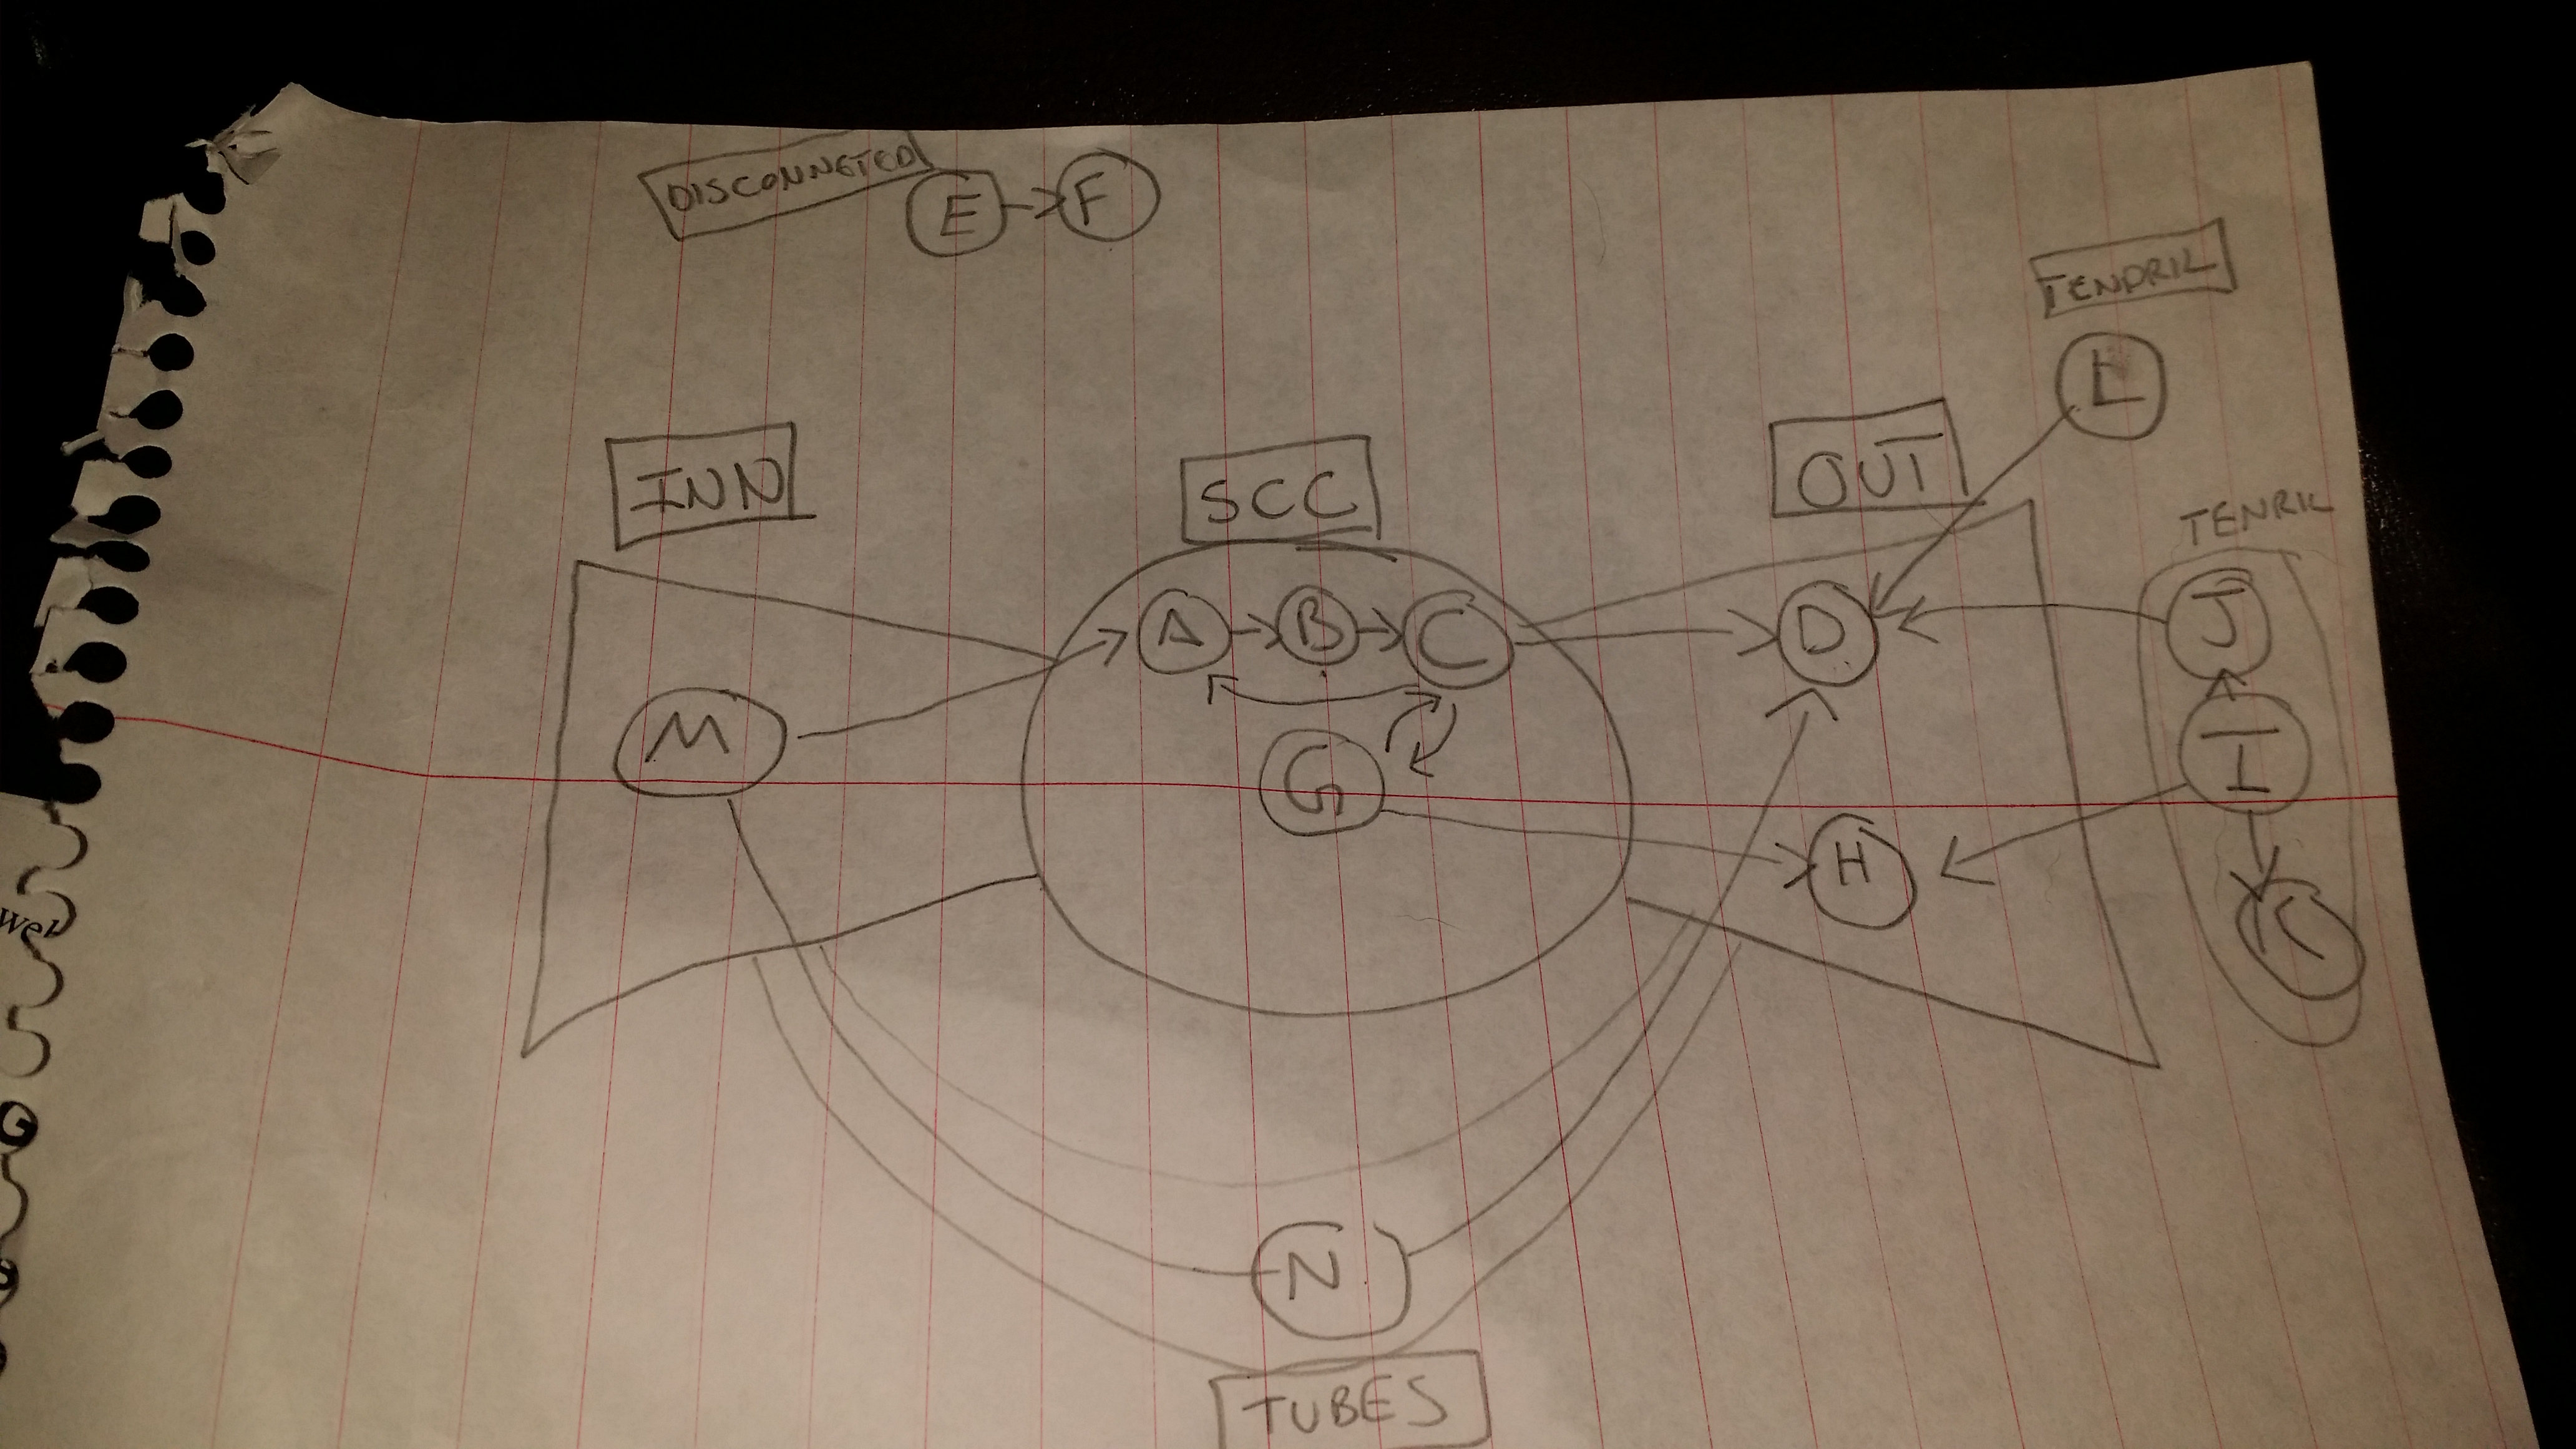
\includegraphics[width=\textwidth]{prob3}
    \caption{Graphical representation in Bow-Tie format}
\end{figure}

{\it Based the Figure 2:}

    IN: {\it M}
    \newline
    SCC: {\it A B C G}
    \newline
    OUT: {\it D H}
    \newline
    Tendrils: {\it J L I K}
    \newline
    Tubes: {\it N}
    \newline
    Disconnected: {\it E F}
    \newline
} 
 
% Stop your text
\end{document}